\documentclass[11pt, a4paper]{article}
% Configuración de márgenes de las páginas
	\usepackage{a4wide}

% Paquete de acentos para Linux
	\usepackage[utf8]{inputenc}

% Paquete para reconocer la separación en sílabas en español
	\usepackage[spanish]{babel}

% Paquetes especiales para el TP
	\usepackage{./otros/caratula}
	\usepackage{pdfpages}

% Paquete para incluir hypervinculos
	\usepackage{color}
	\usepackage{url}
	\definecolor{lnk}{rgb}{0,0,0.4}
	\usepackage[colorlinks=true,linkcolor=lnk,citecolor=blue,urlcolor=blue]{hyperref}

% Paquete para armar índices
	\usepackage{makeidx}
	\makeindex

% Más espacio entre líneas
	\parskip=1.5pt

% Opciones de enumerates
	\usepackage{enumerate}

% Para que las tablas no se muevan libremente
	\usepackage{float}
	\restylefloat{table}

\begin{document}

% Carátula
	\titulo{Aprendizaje por Refuerzos}
	\fecha{2012}
	\materia{Aprendizaje por Refuerzos}
	\integrante{Mariano De Sousa}{??}{marian\_sabianaa@hotmail.com}
	\integrante{Mariano Bianchi}{92/08}{marianobianchi08@gmail.com}
	\integrante{Pablo Brusco}{527/08}{pablo.brusco@gmail.com}
	\maketitle

\section{Problema}
Para este trabajo, se utilizo una versi\'on simplificada del Tower Blocks, el cual se basa en un edificio de bloques al que hay que agregarle nuevos pisos utilizando una gr\'ua. La dificultad radica en que el jugador no puede manejar la gr\'ua, solo puede ejecutar la acci\'on de soltar un nuevo piso sobre el edificio ya construido. De acuerdo a la presici\'on con que se deposite el piso, la torre gana o pierde estabilidad. 
\begin{center} 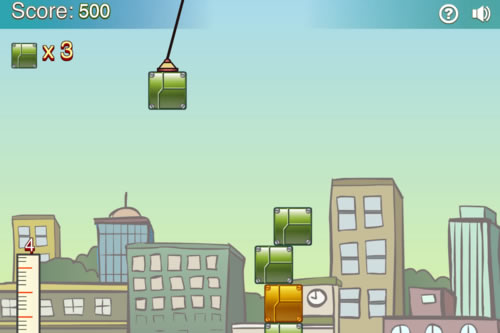
\includegraphics[scale=0.50]{towerblocks}\end{center}

Ya que el juego tiene una gran variedad de niveles y variaciones, se opto por un modelo simple en el cual tenemos que agregar pisos (bloques) a un edificio intentando llegar a una cierta cantidad y sin haber hecho que se derrumbe. Para lo cual existe una gr\'ua que se mueve de manera \textbf{constante} sobre el edificio y nos permite ejecutar la acci\'on de tirar o no tirar. 

\section{Ambiente}
Para la implementaci\'on del ambiente
La grúa es un objeto que tiene un movimiento lineal entre dos posiciones (en este caso -49 y +49), a velocidad constante (1) se mueve en una u otra dirección, de donde se tirará el nuevo piso a agregar. 

Por otro lado, el edificio, posee un movimiento pendular que va variando en velocidad de acuerdo a que tan desbalanceado est\'a, debido a los tiros previos del jugador. 

El ambiente, mantiene un estado visible para el exterior que contiene, la posici\'on y velocidad de la torre, y adem\'as, la posici\'on y direcci\'on de la gr\'ua. 

Dados los parametros que mantiene el ambiente, la cantidad de estados est\'a dada por:
$$ \#estados = \#posiciones\_grua * \#direcciones\_grua * \#posiciones\_torre *  \#velocidad\_torre  $$
Que dada la configuraci\'on que se utilizo, serian:
$$ \# estados = 99 * 2 *99 * 11 = 215622 $$

Aunque no todos ellos son alcanzables dependiendo de otro factor. Este otro factor es el \'angulo m\'aximo que se admite que tenga la torre antes de colapsar y que fuimos variando para encontrar buena dinamica, dejandolo en 30 grados. 

\section{Agentes}
Para implementar los jugadores, utilizamos 2 tipos de agentes. Un agente que aprende utilizando la tecnica de Q-Learning y otro que aprende usando el algoritmo Sarsa-$\lambda$ (ambos utilizando los algoritmos vistos en clase).
Estos agentes, recibian estimulos seg\'un sus posibles acciones: 
\begin{itemize}
\item Tirar
\item Pasar
\end{itemize}
En donde el ambiente podia responder con distintos refuerzos que contemplaban los siguientes casos:
\begin{itemize}
\item Refuerzo por pasar (negativo chico)
\item Refuerzo por fallar y no golpear a la torre (negativo medio)
\item Refuerzo por pegarle a la torre y lograr que se caiga (negativo grande)
\item Refuerzo por tiro  exitoso (golpe\'o la torre y se agreg\'o un nuevo piso)
\end{itemize}


Veamos algunas comparaciones en funci\'on de ciertos parametros que fuimos variando para estudiar 
\subsection{Experimentos}
Para todos los experimentos normalizamos el ambiente para que sea un edificio de 20 pisos al que hay que llegar como objetivo del juego. 

Para responder a las distintas preguntas que uno se puede plantear con respecto a los algoritmos y sus parametros, corrimos los siguientes experimentos:

\bigskip

\begin{table}[h]
\center
\begin{tabular}{ | c | c | c | c | c| }
  \hline
  Agente & $\epsilon$ & $\gamma$ & $\alpha$ & $\lambda$ \\
  \hline 
 	 Q-Learning  & 0.001  & 0.8  & 0.7 & - \\
	Sarsa-$\lambda$  & 0.001  & 0.8  & 0.7 & 0.001 \\
	Sarsa-$\lambda$  & 0.001  & 0.8  & 0.7 & 0.3 \\
	Sarsa-$\lambda$  & 0.001  & 0.8  & 0.7 & 0.7\\
  \hline

\end{tabular}
\caption {Experimento1: Qlearning vs Sarsa-$\lambda$}
\end{table}

\newpage

\subsection{Resultados y Conclusiones}
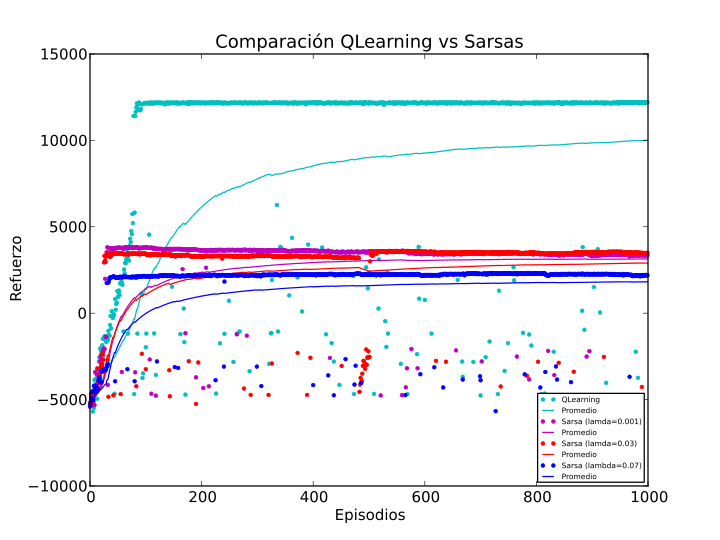
\includegraphics[scale=0.6]{Graf1}

\end{document}